\documentclass[cn,hazy,green,12pt,normal]{elegantnote}

\title{回归分析第一次习题课}
\author{卞泽宇}
\institute{USTC}

\date{\today}

\usepackage{array}

\usepackage{amsmath, amssymb, bm, color, framed, graphicx, hyperref, mathrsfs, fontspec, geometry, extarrows, amsthm}

\DeclareMathOperator{\e}{\!\!\;\mathrm e}
\DeclareMathOperator{\Cov}{Cov}
\DeclareMathOperator{\Var}{Var}
\DeclareMathOperator{\var}{var}
\DeclareMathOperator{\tr}{tr}
\DeclareMathOperator{\diag}{diag}
\newcommand{\p}{\partial}
\renewcommand{\d}{\mathop{}\!\mathrm{d}}
\newcommand{\MR}{\mathbb R}
\newcommand{\MC}{\mathbb C}
\newcommand{\MF}{\mathbb F}
\newcommand{\MZ}{\mathbb Z}
\newcommand{\MN}{\mathbb N}
\newcommand{\MCF}{\mathscr F}
\renewcommand{\Re}{\operatorname{Re}}
\renewcommand{\Im}{\operatorname{Im}}
\renewcommand{\boldsymbol}{\bm}
\renewcommand{\i}{\mathrm i}

\DeclareMathOperator{\Arg}{Arg}
\DeclareMathOperator{\I}{I}
\usepackage{tkz-euclide}
\numberwithin{equation}{section}
\numberwithin{subsection}{section}

\lstset{
    language=R,
    basicstyle=\ttfamily,
    keywordstyle=\color{blue},
    commentstyle=\color{gray},
    frame=single,
    breaklines=true
}

\begin{document}

\maketitle

\tableofcontents

\section{记号说明}
在考量了记号的简洁性,有效性后,我决定之后采用以下记号,并尽量和老师课件保持一致。若有和老师课件不统一之处,请同学仔细甄别。

(1)对于n维随机向量X和m维随机向量Y,记
\begin{enumerate}
    \item 协方差矩阵:$\Sigma_{XY}=\Cov(X,Y)=E[(X-EX)(Y-EY)^T]$,从而$\Sigma_{XY}^T=\Sigma_{YX}$
    \item 方差矩阵:$\Sigma_{XX}=\Var(X)=E[XX^T]-E(X)E(X)^T$
    \item 相关系数矩阵:考察$X=(X_1,X_2,\dots,X_n)$各分量之间的相关性,$D=\diag(\Sigma_{XX})$,则相关系数矩阵$R=D^{-\frac{1}{2}}\Sigma_{XX}D^{-\frac{1}{2}}$
    \item 去相关化矩阵\footnote{之后从投影角度可以知道名称由来}:$\Sigma_{XY \cdot Z}=\Sigma_{XY}-\Sigma_{XZ}\Sigma_{ZZ}^{-1}\Sigma_{ZY}$
\end{enumerate}

(2)对于采样n个样本,p个特征(包含截距)的设计阵$X$,标签$\bm y=(y_1,\dots,y_n)^T$,记
\begin{enumerate}
    \item 均值:$\Bar{\bm x}=\frac{1}{n}\sum_{i=1}^{n}\bm x_i=(m_1,m_2,\dots,m_{p-1})^T\quad$,$\Bar{y}=\frac{1}{n}\sum_{i=1}^{n}y_i$
    \item 中心化(这里X'不表示X的转置):记
    \[
    X'=\begin{bmatrix}
x_{1,1} & x_{1,2}  & \dotsc  & x_{1,p-1} \\
 x_{2,1}&x_{2,2}  &\dotsc  & x_{2,p-1}\\
\vdots  & \vdots  & \ddots  & \vdots \\
x_{n,1} & x_{n,2}  & \dotsc  & x_{n,p-1}
\end{bmatrix}_{n\times (p-1)}\\\ X=[\bm 1, X']
    \]
    $X_c=X'-P_{\bm 1}X'=X'-\bm 1 \frac{1}{n}\sum_{i=1}^{n}\bm x_i^T=X'-\bm 1 \Bar{\bm x}^T=\begin{bmatrix}
        \bm x_1^T-\Bar{\bm x}^T\\
        \bm x_2^T-\Bar{\bm x}^T\\
        \vdots \\
        \bm x_n^T-\Bar{\bm x}^T
    \end{bmatrix}$
    \item $s_{\bm x y}=\sum_{i=1}^{n} (\bm x_i-\Bar{\bm x}) (y_i-\Bar{y})^T=\sum_{i=1}^{n} (\bm x_i-\Bar{\bm x})y_i^T=\sum_{i=1}^{n} \bm x_i (y_i-\Bar{y})^T=X_c^T\bm y \,$ ,$ s_{y \bm x}=s_{\bm x y}^T$
    \item 样本协方差矩阵:$S_{\bm x y}=\frac{1}{n-1}s_{\bm x y}$
    \item 标准化为样本相关系数矩阵:$D=\diag(S_{\bm x\bm x}),R=D^{-\frac{1}{2}}S_{\bm x \bm x}D^{-\frac{1}{2}}$。若令$Z=X_cD^{-\frac{1}{2}}$,则$R=Z^TZ$
    \item $s_{xy\cdot z}=s_{xy}-s_{xz}s_{zz}^{-1}s_{zy}$
\end{enumerate}
\section{作业解答}

\begin{homework}
    假设一物体长度为$\mu$,但$\mu$未知,我们欲估计它,于是将其测量了n次,得到测量值为$y_1,y_2,\dots,y_n$。如果测量过程没有系统误差,我们可以认为$y_i,i=1,\dots,n$为来自正态总体$N(\mu,\sigma^2)$的一组随机样本。试将这些数据表示成线性模型形式。
\end{homework}

\begin{proof}[\solutionname]
    \[ 
    \bm y= \begin{bmatrix}
        y_1\\
        \vdots\\
        y_n
    \end{bmatrix}\quad
    \bm y=\mu \bm 1 + \bm \e \quad
    \bm \e \sim N(\bm 0, \sigma^2 I_n)
    \]
\end{proof}

\begin{note}
    误差项的Gauss-Markov假设
\end{note}

\begin{homework}
    下面的模型是否为一般线性模型?如果不是,能否通过适当的变换使之成为线性模型?

    (1)$Y=\beta_0+\beta_1X_1+\beta_2X_1^2+\beta_3lnX_2+\epsilon$

    (2)$Y=\epsilon \,exp(\beta_0+\beta_1X_1+\beta_2X_1^2)$

    (3)$Y=[1+exp(\beta_0+\beta_1X_1+\epsilon)]^{-\frac{1}{2}}$

    (4)$Y=\beta_0+\beta_1(X_1+X_2)+\beta_2e^{X_1+X_2}+\beta_3lnX_1^2+\epsilon$
\end{homework}
\begin{proof}[\solutionname]
    (1)是。

    (2)不是,两侧取绝对值,再取对数,令$\tilde{Y}=ln |Y|,\tilde{\epsilon}=ln|\epsilon|,\tilde{X_2}=X_1^2$变换为线性模型.

    (3)不是,先两侧平方,取倒数,同时减1,再取对数。令$\tilde{Y}=ln(Y^{-2}-1)$得。
\end{proof}

(4)是。

\begin{note}
    重点看是否对参数线性。
\end{note}

\begin{homework}
    写出二元线性回归模型,并参考教学课件第一章第一节p20 Table1.1中矫正叉积矩阵符号给出回归系数的最小二乘(OLS)估计。
\end{homework}
\begin{proof}[\solutionname]
\[
    \bm y = \alpha \bm 1_n+X_c \bm \beta_c +\bm e
    \]
    其中p=3。由公式得$\hat{\alpha}=\Bar{y}$,$\hat{\bm \beta_c}=(X_c^TX_c)^{-1}X_c^T\bm y$,
    \[
    \hat{\bm \beta_c}=
    \begin{bmatrix}
        SX_1X_1&SX_1X_2\\
        SX_2X_1&SX_2X_2\\
    \end{bmatrix}^{-1}\begin{bmatrix}
        (X_1-\bm 1 m_1)^T\\
        (X_2-\bm 1 m_2)^T\\
    \end{bmatrix}\bm y
    =\begin{bmatrix}
        SX_1X_1&SX_1X_2\\
        SX_2X_1&SX_2X_2\\
    \end{bmatrix}^{-1}\begin{bmatrix}
        SX_1Y\\
        SX_2Y
    \end{bmatrix}\]
\end{proof}

\begin{homework}
    为考察某种维尼纶纤维的耐水性,安排了一批实验,测得甲醛浓度X及"浓缩化度"Y的数据如下:
    
\begin{tabular}{|l|l|l|l|l|l|l|l|}
\hline
X & 18    & 20    & 22    & 24    & 26    & 28 & 30    \\ \hline
Y & 26.86 & 28.35 & 28.75 & 28.87 & 29.75 & 30 & 30.36 \\ \hline
\end{tabular}

从实际经验及理论知识假设两者近似线性关系。求Y关于X的OLS拟合回归方程,并借助R或Python画出散点图和拟合回归直线。
\end{homework}
\begin{proof}[\solutionname]

\begin{lstlisting}
x <- seq(18, 30, by=2)
y <- c(26.86, 28.35, 28.75, 28.87, 29.75, 30, 30.36)
model <- lm(y ~ x)
plot(x, y, xlab = "X", ylab = "Y")  # draw a picture
abline(model)
summary(model)  # view details
    \end{lstlisting}
\end{proof}

\begin{figure}[!htbp]
    \centering
    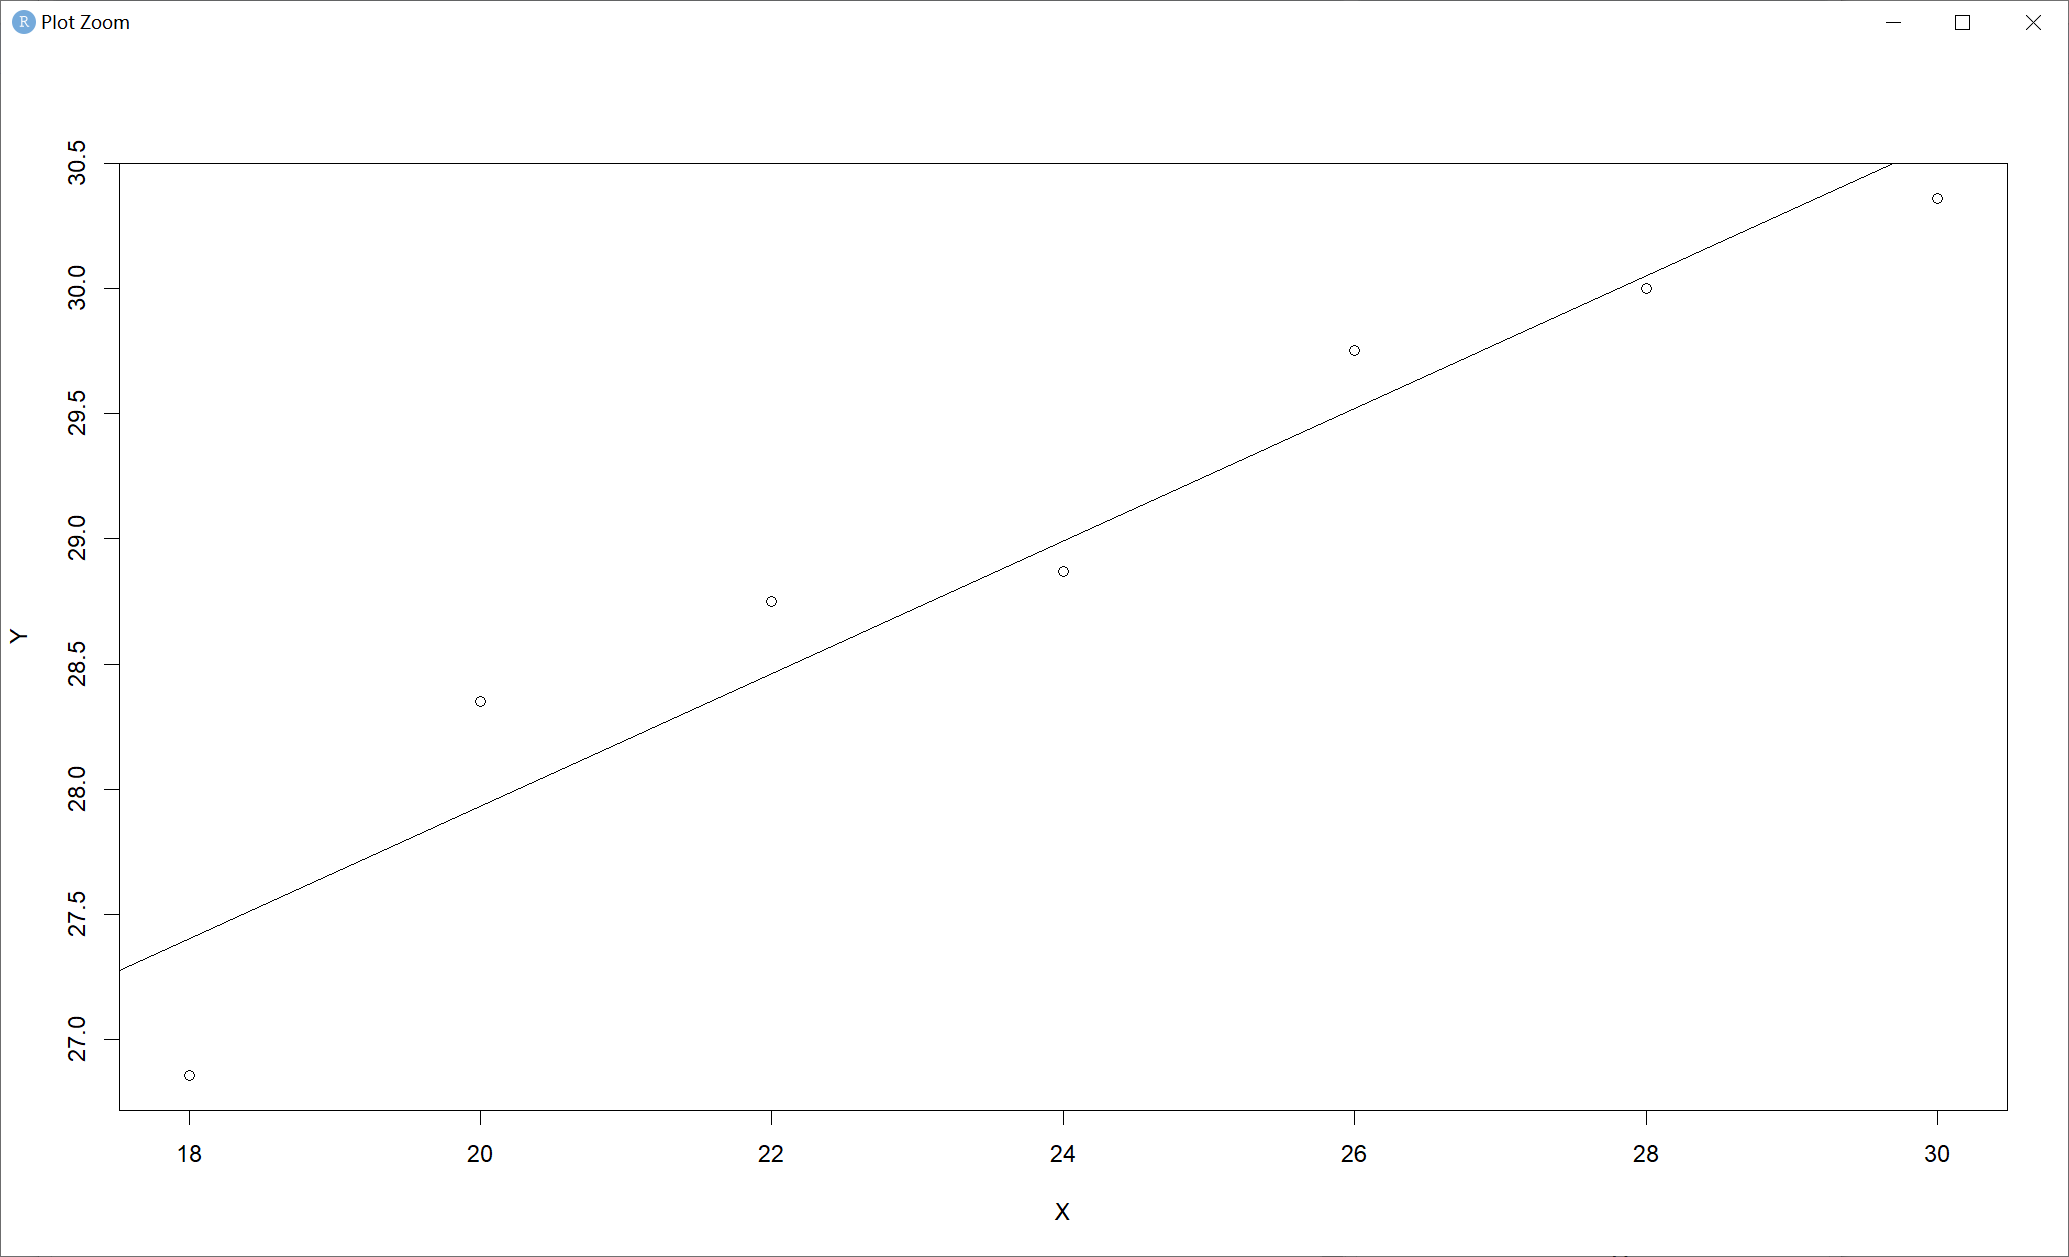
\includegraphics[width=28em]{image/ex1_plt1.png}
\end{figure}
\begin{homework}
    对于正态线性回归模型
\[\bm y=X\bm \beta +e, \qquad e \sim N(0,\sigma^2 I_n)\]
给出参数向量$\beta$的极大似然估计,并与OLS比较。
\end{homework}
\begin{proof}[\solutionname]
    参数向量$\bm \beta$的似然函数:
    $$
    L(\bm \beta )=(2\pi \sigma^2)^{-\frac{n}{2}} exp\{-\frac{1}{2\sigma^2}(\bm y-X\bm \beta)^T(\bm y-X\bm \beta)\}
    $$
    求解似然函数$L(\bm \beta)$的最大值等价于求解如下函数的最小值:
    $$
    Q(\bm \beta) = (\bm y-X\bm \beta)^T(\bm y-X\bm \beta)
    $$
    对$\bm \beta$求导,并令导数为0,得:
    $$
    \dfrac{\p Q}{\p \bm \beta}=2X^T(X\bm \beta -\bm y)
    $$
    故$\hat{\bm \beta}_{MLE}=(X^TX)^{-1}X^T\bm y$.

    证明上述$\hat{\bm \beta}_{MLE}$确实使$Q(\bm \beta)$达到最小值。一种方法是验证Hessian矩阵$\dfrac{\p^2 Q}{\p \bm \beta \bm \beta^T}=2X^TX$为半正定矩阵。另一种方法是:
    $$
    \begin{aligned}
         Q(\bm \beta) &= \Vert \bm y-X\bm \beta \Vert_2^2 \\
         &= \Vert \bm y- X\hat{\bm \beta}_{MLE} + X\hat{\bm \beta}_{MLE} -X\bm \beta \Vert_2^2 \\
         &= \Vert \bm y- X\hat{\bm \beta}_{MLE} \Vert_2^2 + \Vert X\hat{\bm \beta}_{MLE} -X\bm \beta \Vert_2^2 + (\bm y- X\hat{\bm \beta}_{MLE})^T(X\hat{\bm \beta}_{MLE} -X\bm \beta) \\
         &= \Vert \bm y- X\hat{\bm \beta}_{MLE} \Vert_2^2 + \Vert X\hat{\bm \beta}_{MLE} -X\bm \beta \Vert_2^2 \\
         &\geq \Vert \bm y- X\hat{\bm \beta}_{MLE} \Vert_2^2
    \end{aligned}
    $$
    其中等式第三行最后一项为0。故$\hat{\bm \beta}_{MLE}$确实使$Q(\bm \beta)$达到最小值。

    参数向量$\bm \beta$的极大似然估计与OLS估计的结果是一样的。
\end{proof}
\begin{note}
    求导并令导数为0后需进一步验证$\hat{\bm \beta}_{MLE}$确实使$Q(\bm \beta)$达到最小值。注意到求解过程实际在求$\min_{\bm \beta} (\bm y-X\bm \beta)^T(\bm y-X\bm \beta)$,与OLS目标相同。若$X^TX$不可逆就用广义逆代替。
\end{note}

\begin{homework}
    对于简单线性回归模型$Y=\beta_0+\beta_1X+e$,考虑回归变量为随机变量。假设$(x_1,y_1),\dots,(x_n,y_n)\quad i.i.d. \sim N(\mu, \Sigma)$,其中
    \[
    \mu=\begin{bmatrix}
        \mu_x\\
        \mu_y
    \end{bmatrix}
    \quad
    \Sigma=\begin{bmatrix}
        \sigma_x^2 & \rho\sigma_x\sigma_y\\
        \rho\sigma_x\sigma_y & \sigma_y^2
    \end{bmatrix}
    \]
    请给出$\beta_1$关于$\mu,\Sigma$的表达式,并给出$\rho $的一个估计量。
\end{homework}
\begin{proof}[\solutionname]
\[
    \rho\sigma_x\sigma_y=\Cov(X,Y)=\Cov(X,\beta_0+\beta_1X+e)=\beta_1\Cov(X,X)=\beta_1\sigma_x^2 \Rightarrow \beta_1=\rho\frac{\sigma_y}{\sigma_x}
    \]
    取Pearson相关系数作为$\rho$估计:$r=\hat{\beta_1}\dfrac{\hat{\sigma_x}}{\hat{\sigma_y}}=\dfrac{SXY}{\sqrt{SXX\cdot SYY}}$
\end{proof}
\begin{note}
    这里是总体模型,注意区分参数和估计量。
\end{note}
\begin{homework}
    设
    \[
    \begin{aligned}
    y_1&=\theta+e_1\\
    y_2&=2\theta-\varphi +e_2\\
    y_3&=\theta+2\varphi +e_3\\
    \end{aligned}
    \]
    其中$\theta,\varphi$为未知参数。$E(e_i)=0,Var(e_i)=\sigma^2,\forall i$,且$e_i$相互独立。

    (a)求$\theta,\varphi$的最小二乘估计$\hat{\theta},\hat{\varphi}$;

    (b)求$\Cov\begin{bmatrix}
        \hat{\theta}\\
        \hat{\varphi}
    \end{bmatrix}$
\end{homework}
\begin{proof}[\solutionname]
   (a) 记\[
    \bm \beta = \begin{bmatrix}
        \theta\\
        \varphi
    \end{bmatrix},\quad \bm y = \begin{bmatrix}
        1&0\\
        2&-1\\
        1&2\\
    \end{bmatrix}\bm \beta +\bm e
    \]
    代入公式即得。

    (b)利用$\Cov(\bm \hat{\beta})=\sigma^2(X^TX)^{-1}$
\end{proof}
\begin{homework}
    设\[
    \begin{aligned}
        &y_i=\theta +e_i, \quad i=1,\dots,m\\
        &y_{m+j}=\theta +\varphi +e_{m+j}\quad j=1,\dots,m\\
        &y_{2m+k}=\theta -2\varphi +e_{2m+k},\quad k=1,\dots,n
    \end{aligned}
    \]
    其中$\theta,\varphi$为未知参数,$e_i\quad i.i.d. \sim N(0,\sigma^2)$。

    (a)写出设计阵X

    (b)求$\theta,\varphi$的最小二乘估计$\hat{\theta},\hat{\varphi}$

    (c)证明当m=2n时,$\hat{\theta}$与$\hat{\varphi}$不相关。
\end{homework}
\begin{proof}[\solutionname]
    类似作业7,代入公式求解即可,第三问考虑两者协方差。
\end{proof}

\begin{homework}
    已知$X\sim N_n(\bm \mu, I_n )$

    (a)求$Y_1=\bm a ^T X$和$Y_2=\bm b^T X$的联合分布,其中$\bm a, \bm b$为$n\times 1$常向量,且不共线。

    (b)若$\bm a^T \bm b=0$,证明$Y_1,Y_2$独立。
\end{homework}

\begin{proof}
    (a) 记$A=\begin{bmatrix}
        \bm a^T\\
        \bm b^T\\
    \end{bmatrix}$行满秩,考虑$AX\sim N_2(A\mu,AA^T)$
    
    (b)从联合分布可知,此时协方差阵为对角阵。多元正态不相关进而独立。
\end{proof}

\begin{homework}
    设$X\sim N_n(\bm \mu, \Sigma),A$是$n\times n$对称矩阵,证明当$A\Sigma A=A$时,$(X-\bm \mu )^TA(X-\bm \mu)\sim \chi_r^2,r=Rank(A)$
\end{homework}
\begin{proof}
    由于$\Sigma$为正定阵,故$A=A\Sigma A=A\Sigma A^T$半正定
    \begin{figure}[!htbp]
        \centering
        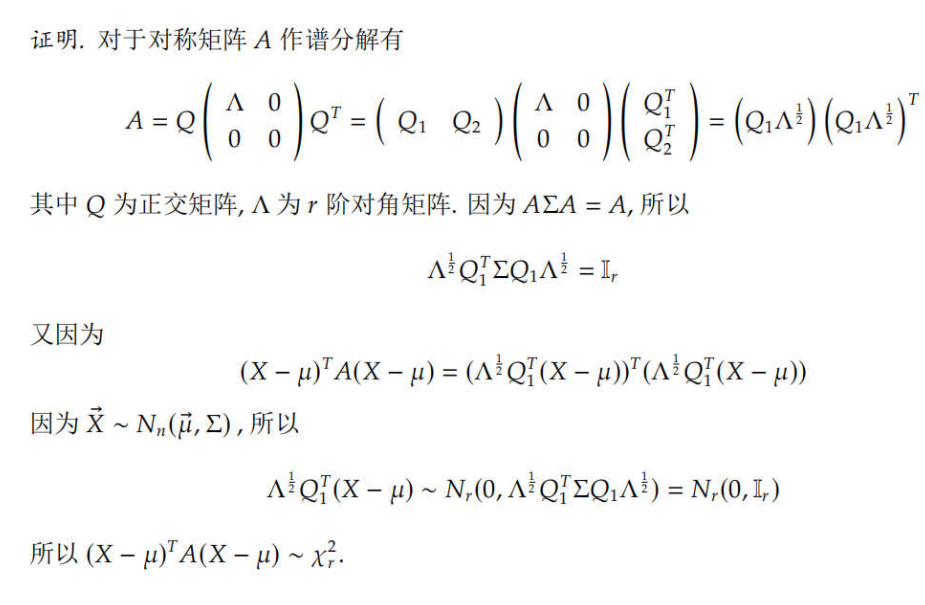
\includegraphics[width=30em]{image/ex1_plt2.png}
    \end{figure}
    
\end{proof}
    
\begin{homework}
    对于简单线性回归模型:
    \[y_i=\beta_0+\beta_1x_i+e_i\]满足Gauss-Markov假设,验证通过OLS得到的拟合回归直线其残差平方和
    \[RSS=SYY-\dfrac{(SYY)^2}{SXX}\],
    并证明测定系数$R^2$等于因变量Y与自变量X之间样本相关系数的平方,即
    \[R^2=\dfrac{(SXY)^2}{SXX\cdot SXY}\]
\end{homework}
\section{代码补充}

\subsection{Introduction to R}
R is a language and environment for statistical computing and graphics.

R provides a wide variety of statistical (linear and nonlinear modelling, classical statistical tests,  time-series analysis, classification, clustering, \dots) and graphical techniques, and is highly extensible.

You may consider R as an environment within which statistical techniques are implemented instead of a statistics system. R can be extended (easily) via packages. There are about eight packages supplied with the R distribution and many more are available through the CRAN family of Internet sites covering a very wide range of modern statistics.

\textbf{Download: https://cran.r-project.org/mirrors.html}
\vspace*{-1em}

\hspace{4.7em} \textbf{https://mirrors.ustc.edu.cn/CRAN/}
\subsection{Introduction to RStudio}
You are \textbf{highly recommended} to install RStudio. The R programming language comes with its own basic user interface that is adequate for modest applications. But larger applications become unwieldy in the basic R user
interface, and therefore it helps to install a more sophisticated R-friendly editor \, :)

RStudio is an integrated development environment (IDE) for R and Python. It includes a console, syntax-highlighting editor that supports direct code execution, and tools for plotting, history, debugging, and workspace management. RStudio is available in open source and commercial editions and runs on the desktop (Windows, Mac, and Linux).

\textbf{Download: https://posit.co/download/rstudio-desktop/} 

After you have successfully installed R and RStudio, you \textbf{only} need to open RStudio everytime you code.

For more information and tutorials, you can refer to
\vspace{-1em}

\hspace{-2em}\textbf{https://www.math.pku.edu.cn/teachers/lidf/docs/Rbook/html/\_Rbook/index.html}

Don't get bothered by the massive contents, you are only required to be familiar with some basic usages and 
commands (e.g. we use '<-' instead of '=' when assigning variable values, you can type in '<-' with the hotkey 
'Alt' + '-')

I will also display some codes based on RStudio in the following exercise class lecture notes.
\begin{example}[relations with other software tools]
    \begin{figure}[!htbp]
    \centering
    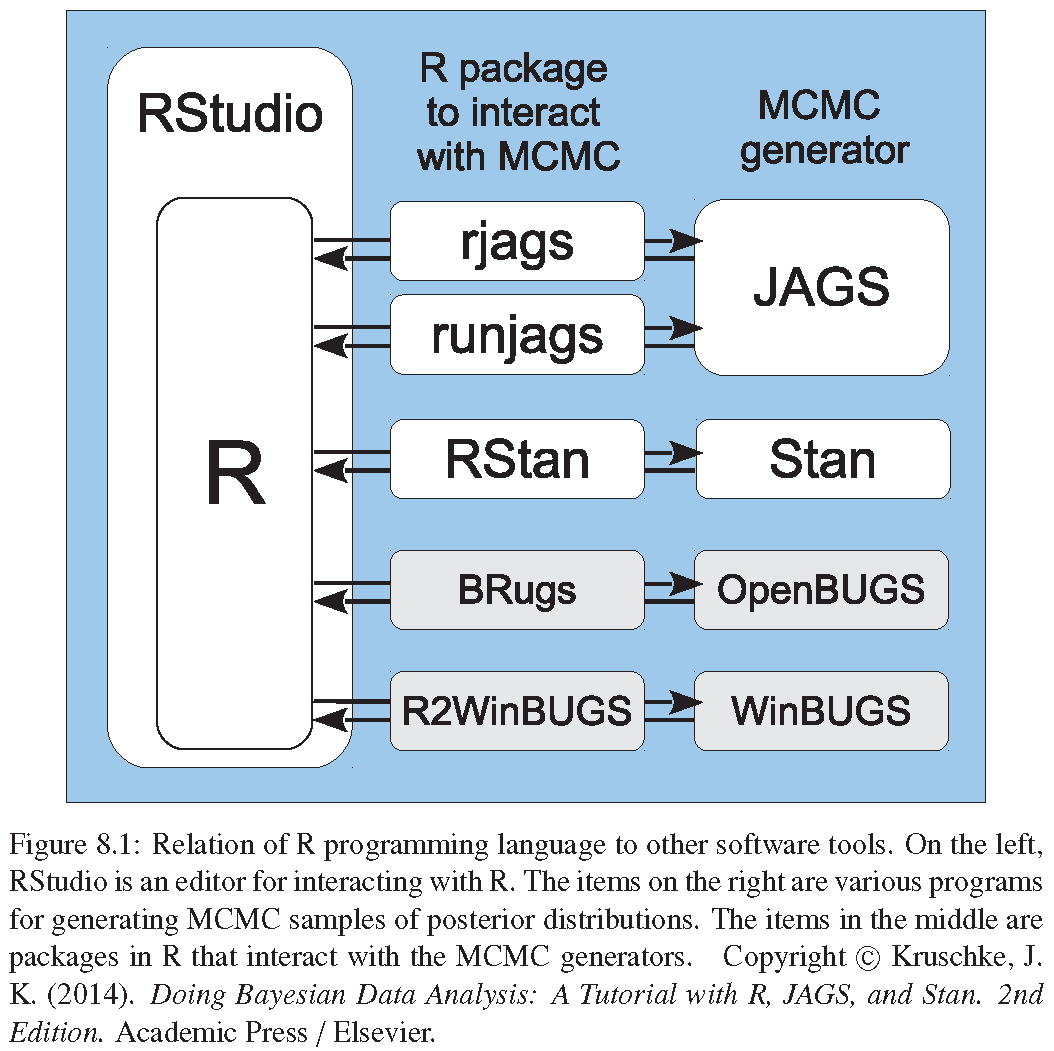
\includegraphics[width=24em]{./image/image_1.png}
    \label{image_1}
\end{figure}
\end{example}

\subsection{相关分析实验}
参考群文件lab 1。
% \begin{lstlisting}[language=R, caption={}]
% x<-c(1,2,3)  # 创建一个向量
% sum(x)
% \end{lstlisting}

\section{额外内容补充}
\subsection{总体线性模型}
总体模型是指在采样前,对几个随机变量中的关系进行建模。而线性模型主要指关于参数线性,比如$y=a x^2+b x+c+\e$可以看作是对参数$(a,b,c)$的线性模型。

总体模型$y=a+\bm x^T \bm b+\e$下的Gauss-Markov假设:
\begin{enumerate}
    \item 截距可识别:$E(e)=0$
    \item 方差齐性:$var(\e)=\sigma^2$
    \item 外生性: $\e \text{与}\bm x$独立
\end{enumerate}
其中第三条说明$\e$不是confounder,是推断因果必需的。
\subsection{投影角度看待条件期望}
假设概率空间$(\Omega,\MCF,P)$,记$L^2(\Omega)$为其上平方可积实值随机变量构成的内积空间\footnote{视a.s.相等为恒等,并且为Hilbert space。见https://math.stackexchange.com/questions/1383460解答
}(i.e. $E[X^2]<\infty$全体),赋予内积$\langle X,Y \rangle=E(XY)$。则
\begin{proposition}

\begin{enumerate}
    \item  给定$X,Y \in L^2(\Omega)$,考虑$(\hat{a},\hat{b})=\arg \min_{a,b} E[(Y-a-bX)^2]$。则这个最优解称为线性最小平方估计(LLSE, linear least squares estimator)。记$\hat{Y}=\hat{a}+\hat{b}X$,则
    
    \[
\hat{Y}=L(Y|X)=EY+\Sigma_{YX}\Sigma^{-1}_{XX}(X-EX)
    \]
    \item 设$X,Y \in L^2(\Omega)$,求$\hat{f}(X)=\arg \min_{f} E[(Y-f(X))^2]$。这个解称为最小均方误差估计(MMSE, minimum mean square error estimator)。这个解是存在唯一的,即条件期望$E(Y|X)$。
\end{enumerate}
\end{proposition}

\begin{proof}
    (1)由泛函分析知,即求$Y$往$V=span\{\bm 1,X\}$上的投影$L(Y|X)=P_V Y$。这个投影存在唯一,满足:
 \[\begin{cases}
        0=\langle \bm 1,Y-\hat{Y}\rangle=E[Y-\hat{Y}],\\
        0=\langle X,Y-\hat{Y}\rangle = E[X(Y-\hat{Y})].
    \end{cases}\]
    代入求解得:
     \[\begin{cases}
       \hat{b}=\Sigma_{YX}\Sigma_{XX}^{-1},\\
       \hat{a}=EY-\hat{b}EX.
    \end{cases}\]

    (2)考虑$E[(Y-f(X))^2|X]$,
    \[
\begin{aligned}
    E[(Y-f(X))^2|X]&=E[(Y-E[Y|X]+E[Y|X]-f(X))^2|X]\\    
    &=E[(Y-E[Y|X])^2|X]+2E[(Y-E[Y|X])(E[Y|X]-f(X))|X]\\&\hspace{1em}+E[(E[Y|X]-f(X))^2|X]\\
    &=E[(Y-E[Y|X])^2|X]+(E[Y|X]-f(X))^2\\
    &\ge E[(Y-E[Y|X])^2|X]
\end{aligned}
\]
进而两边对$X$取期望得到下界$E[(Y-E[Y|X])^2]$,取等当且仅当$f(X)=E[Y|X]$。
\end{proof}
\begin{note}
    (1)也可以考虑$Y$往$span\{\bm 1, X, X^2,\dots,X^d\}$空间投影,同样列出方程组不难求解。只不过这时候要求$X^d \in L^2(\Omega)$(i.e. $E(X^{2d}<\infty$))
    
    \noindent (2)上述结果可以推广到n维随机向量$X$和m维随机向量$Y$。解的形式相同,见\ref{decorrelation}

    \noindent (3)以上只是我的一些想当然推导,参考了一点资料,可能会有缺少条件或者不严谨之处,望指正。
\end{note}
\begin{example}[C-R下界,参考上学期教材p110]
    设$\MCF=\{f(x,\theta),\theta \in \Theta\}$为C-R正则分布族,$g(\theta)$为定义在空间$\Theta$上的可微函数。设样本$X=(X_1, \dots,X_n)$为由总体中抽取的简单随机样本。$\hat{g}(X)$为$g(\theta)$的任意无偏估计,且满足积分号下求导条件,则
    \[
    D_{\theta}[\hat{g}(X)]\ge \dfrac{(g'(\theta ))^2}{nI(\theta)} \qquad \forall \theta \in \Theta
    \]
\end{example}
\begin{proof}
    设$S(\bm x,\theta)=\dfrac{\p log f(\bm x,\theta)}{\p \theta}$
    
    可求得$E[S(\bm x,\theta)]=0,\Cov(\hat{g}(X),S(\bm x,\theta))=g'(\theta), D_{\theta}(S(\bm x,\theta))=nI(\theta)$

    考虑$\hat{g}(X)$往$span\{S(\bm x,\theta)\}$上的线性投影$L(\hat{g}(X)|S(\bm x,\theta))$,其方差即为$\dfrac{(g'(\theta ))^2}{nI(\theta)}$,自然有$\Var(\hat{g}(X))\ge \Var(L(\hat{g}(X)|S(\bm x,\theta)))$

    并且可以发现为什么有时UMVUE方差是达不到C-R下界的:假设若$S(\bm x,\theta)$为充分完全统计量,则其分布与$\theta$无关。此时$E(\hat{g}(X)|S(\bm x,\theta))$为往$L^2(\sigma(S(\bm x, \theta)))$上的投影。由L-S定理知,此投影不依赖于参数,且为UMVUE。
    
    另一方面,由于$span\{\bm 1, S(\bm x, \theta)\} \subseteq L^2(\sigma(S(\bm x, \theta)))$,因此对应UMVUE的方差可能严格大于C-R下界。

    从中也可以发现C-R下界就是找了个有比较好性质的枢轴量,计算某无偏估计向向其的线性投影。
\end{proof}

\begin{example}
    证明:$\Var(\bm y)=\Var[E(\bm y|\bm x)]+E[\Var(\bm y|\bm x)]$
\end{example}
\begin{proof}
    参考\cite{cn3} HW5,练习4.1
\end{proof}
\subsection{去相关化}\label{decorrelation}
不妨假设n维随机向量$X$,m维随机向量$Y$已经中心化。希望求取$A\in \MR^{m\times n}$,使$X$与$Y-AX$不相关,即$\Cov(X,Y-AX)=0$。

利用$0=\Cov(X,Y-AX)=\Sigma_{XY}-\Sigma_{XX}A^T$,得$A=\Sigma_{YX}\Sigma_{XX}^{-1}$。

记$\hat{Y}=\Sigma_{YX}\Sigma_{XX}^{-1}X\quad$,$Y^{\perp}=Y-\hat{Y}=Y-\Sigma_{YX}\Sigma_{XX}^{-1}X$

\begin{figure}[!htbp]
    \centering
    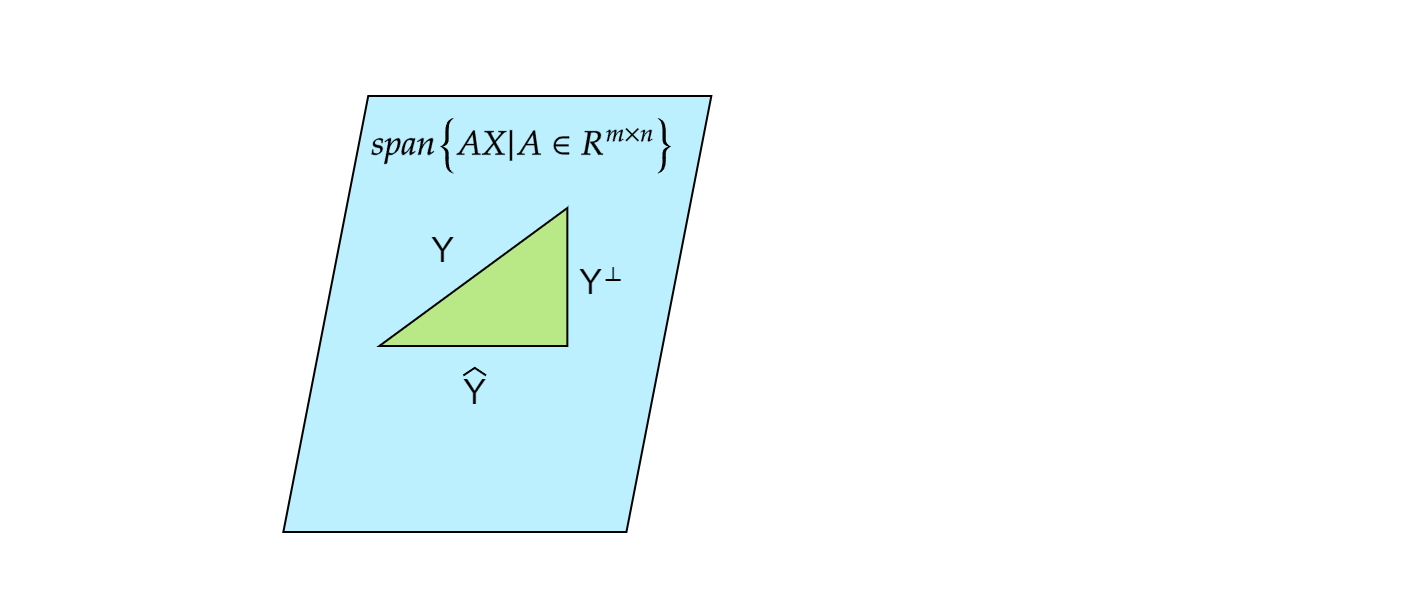
\includegraphics[width=40em]{image/image_2.png}
    \label{image_2}
\end{figure}

$Y^{\perp}$称为$Y$关于$X$的去相关化,且有:
\begin{proposition}\label{p1}
    \begin{enumerate}
        \item $\Var(\hat{Y})=\Sigma_{YX}\Sigma_{XX}^{-1}\Sigma_{XY}$
        \item  $\Var(Y^{\perp})=\Var(Y)-\Var(\hat{Y})=\Sigma_{YY}-\Sigma_{YX}\Sigma_{XX}^{-1}\Sigma_{XY}=\Sigma_{YY\cdot X}$
        \item $E[||Y-\hat{Y}||^2]=\tr(E[(Y-\hat{Y})^T(Y-\hat{Y})])=E[\tr((Y-\hat{Y})(Y-\hat{Y})^T)]=\tr(\Var(Y^{\perp}))$
    \end{enumerate}
\end{proposition}

\begin{proposition}
    假设总体模型$y = a+\bm x^T b+e$,$E(e)=0$,$\var(e)=\sigma^2$,$e\text{与}\bm x$独立,则$a,b,\sigma^2$由$y,\bm x$的均值、方差决定,具体如下:
    \begin{enumerate}
        \item $b=\Sigma_{\bm x \bm x}^{-1}\Sigma_{\bm x y}$
        \item $a=\mu_{y}-\mu_{\bm x}^T b$
        \item $\sigma^2=\Sigma_{yy\cdot \bm x}=\Sigma_{yy}(1-\Phi)$
        \item $\Phi:=\dfrac{\var(\bm x^T b)}{\var (y)}=\dfrac{\Sigma_{y\bm x}\Sigma_{\bm x\bm x}^{-1}\Sigma_{\bm x y}}{\Sigma_{yy}}$,称为决定系数。
    \end{enumerate}
\end{proposition}
\begin{proof}
    (1)由于$e=y-a-\bm x^Tb$与$\bm x$独立,说明$e$为$y$关于$\bm x$的去相关化,因此由去相关化公式得$b^T=\Sigma_{y\bm x}\Sigma_{\bm x\bm x}^{-1},b=\Sigma_{\bm x \bm x}^{-1}\Sigma_{\bm x y}$

    \noindent (2)对模型两侧取期望,即得$a=\mu_{y}-\mu_{\bm x}^T b$
    
    \noindent (3)由$e=y^{\perp}$,故由\ref{p1}得$\sigma^2=\var(e)=\Sigma_{yy\cdot \bm x}$

    \noindent (4)第一个等式为定义,从几何角度来看为$\Phi=\cos^2(\theta)=\dfrac{\var(\hat{y})}{\var(y)}=\dfrac{\Sigma_{y\bm x}\Sigma_{\bm x\bm x}^{-1}\Sigma_{\bm x y}}{\Sigma_{yy}}$
\end{proof}
\begin{example}[线性回归模型的矩估计]
    假设样本满足线性回归方程$\bm y=X\bm \beta +\bm e=\beta_0+Z\bm \beta_1+\bm e$,且满足G-M假设。则参数的矩估计为:
    \[
    \begin{cases}
        \tilde{\bm \beta_1}=s_{\bm x \bm x}^{-1}s_{\bm x\bm y}=S_{\bm x \bm x}^{-1}S_{\bm x\bm y},\\
        \tilde{\beta_0}=\Bar{\bm y}-\Bar{\bm x}^T \hat{\bm \beta_1},\\
        \tilde{\sigma^2}=S_{\bm y\bm y\cdot \bm x},\\
        R^2=\tilde{\Phi}=\dfrac{S_{y\bm x}S_{\bm x\bm x}^{-1}S_{\bm x y}}{S_{yy}}
    \end{cases}
    \]
    可以注意到,除了$\tilde{\sigma^2}$与LS估计不同,其余的估计和LS结果是一致的。
    设$\hat{\sigma^2}$为对应LS估计,则$\hat{\sigma^2}=\dfrac{n-1}{n-p}\tilde{\sigma^2}\approx \tilde{\sigma^2}$,常数的不同是为了保证LS估计无偏性。
\end{example}

\subsection{投影矩阵}
我们知道,在Hilbert空间中幂等和自共轭性质等价于其为投影算子。放到有限维欧氏空间中,对应一定的投影矩阵(紧算子)。
记矩阵$A\in \MR^{m\times n}$的列空间为$C(A)$
\subsection[标量对矩阵求导]{标量对矩阵求导\cite{cn1}}
以下主要介绍标量对于向量或者矩阵求导的计算技巧。向量用黑体$\bm x$表示,如无特殊说明,默认为列向量。

我们已经在数分A2中接触过标量函数自变量(可以是高维),得到函数的梯度。其关键在于视每个分量为独立的,
对每个分量求偏导后,按一定顺序拼在一起得到的向量即为梯度。不过到底是行向量还是列向量依赖于通俗的规定。

下面介绍两种布局:
\begin{itemize}
    \item 分子布局:导数维度以分子为主
    \item 分母布局:导数维度以分母为主
\end{itemize}
可见这两种布局始终\textbf{相差一个转置}。

比如m维向量$\bm y$对n维向量$\bm x$求导,
分子布局将矩阵的第一个维度(行)以分子$\bm y$为准,结果为
\[
\frac{\p \bm y}{\p \bm x} = \begin{bmatrix}
\frac{\p y_1}{\p x_1} &\frac{\p y_1}{\p x_2}  & \dotsc  & \frac{\p y_1}{\p x_n} \\
 \frac{\p y_2}{\p x_1}&\frac{\p y_2}{\p x_2}  &\dotsc  & \frac{\p y_2}{\p x_n}\\
\vdots  & \vdots  & \ddots  & \vdots \\
\frac{\p y_m}{\p x_1} & \frac{\p y_m}{\p x_2}  & \dotsc  & \frac{\p y_m}{\p x_n}
\end{bmatrix}_{(m\times n)}
\]
类似的,分母布局则以$\bm x$为准,结果为

\[
\frac{\p \bm y}{\p \bm x} = \begin{bmatrix}
\frac{\p y_1}{\p x_1} &\frac{\p y_2}{\p x_1}  & \dotsc  & \frac{\p y_m}{\p x_1} \\
 \frac{\p y_1}{\p x_2}&\frac{\p y_2}{\p x_2}  &\dotsc  & \frac{\p y_m}{\p x_2}\\
\vdots  & \vdots  & \ddots  & \vdots \\
\frac{\p y_1}{\p x_n} & \frac{\p y_2}{\p x_n}  & \dotsc  & \frac{\p y_m}{\p x_n}
\end{bmatrix}_{(n\times m)}
\]

若f是矩阵$A\in \MF^{m\times n}$的标量函数,f=f($A$),则分母布局为:
\[
\frac{\p f}{\p A} = \begin{bmatrix}
\frac{\p f}{\p a_{11}} &\frac{\p f}{\p a_{12}}  & \dotsc  & \frac{\p f}{\p a_{1n}} \\
 \frac{\p f}{\p a_{21}}&\frac{\p f}{\p a_{22}}  &\dotsc  & \frac{\p f}{\p a_{2n}}\\
\vdots  & \vdots  & \ddots  & \vdots \\
\frac{\p f}{\p a_{m1}} & \frac{\p f}{\p a_{m2}}  & \dotsc  & \frac{\p f}{\p a_{mn}}
\end{bmatrix}_{(m\times n)}
\]
为按照各元素求偏导后排成的矩阵,维度和$A$一致。

在之后的推到中,我们采取以下布局约定:
\begin{itemize}
    \item 向量或者矩阵对标量求导时,采取分子布局。
    \item 标量对向量或矩阵求导时,采取分母布局。
    \item 向量对向量求导时,采取分子布局。
\end{itemize}

\begin{note}
    前两条我们应该比较熟悉,看起来也挺合理。第三条和我们数分A2讲解的向量值函数Jacobi矩阵是一致的,
    我们也能运用对应的复合求导法则而不至于弄错顺序。

    \noindent 但注意A2中的梯度一般为行向量,复合求导要小心。这里按照约定应该为列向量,这和运筹学是一致的。
\end{note}

\begin{example}{复合求导法则:}
    设向量值函数$\bm f \in \MR^m$为关于$\bm x \in \MR^n$的函数,$\bm x = \bm x(y_1,y_2,
    \dots, y_d)$为关于$\bm y \in \MR^d$函数。求$\Tilde{\bm f}(\bm y)=\bm f(\bm x(\bm y))$关于$\bm y$的Jacobi阵。
\end{example}

\begin{proof}[\solutionname]
\[
    \frac{\p \Tilde{\bm f}}{\p \bm y} = \frac{\p \bm f}{\p \bm x}\bigg|_{\bm x_0} \frac{\p \bm x}{\p \bm y}\bigg|_{\bm y_0}
\]
其中$\bm x_0=\bm x(\bm y_0)$,结果为$m\times n$和$n\times d$两个矩阵的乘积,最终维数为$m \times d$ (可验证出现的所有Jacobi阵均为分子布局)
\end{proof}

下面我们来推导快速计算导数的公式,假设f为标量函数,$\bm x$为n维向量。
注意到一次微分形式$\d f$可以写成对偶基$\{\d x_i\}_{i=1,\dots,n}$的线性组合:$\d f = \sum_{i=1}^n
\frac{\p f}{\p x_i} \d x_i = (\nabla f)^T \d \bm x$。
因此我们或许可以通过求解全微分,再从某种内积结构中提取出导数。

我们知道,$\tr(A^T B)$可以是定义在内积空间$(\MR^{m\times n}, \MR)$上的一个内积,并且诱导矩阵Frobenius范数。因此我们设计以下步骤\footnote{利用上述提示自证不难}求解Jacobi导数:

step 1: 求解$\d f$
\vspace{-1em}

step 2: 两边套上tr(),注意到标量函数$\tr(\d f) = \d f$
\vspace{-1em}

step 3: 根据tr()的一些性质化简出$\d f = \tr((\frac{\p f}{\p A})^T \d A)$

即得到了$\dfrac{\p f}{\p A}$。

\begin{example}
$y= \bm a^T X \bm b$,$\bm a$和$\bm b$分别为m,n维向量,$X$为$m\times n$维矩阵,求$\dfrac{\p y}{\p X}$
\end{example}

\begin{proof}[\solutionname]
    法1:按照定义法,有
    \[
    y = \sum_{i,j} a_i x_{ij} b_j
    \]
    因此$\dfrac{\p y}{\p X}\bigg|_{(i,j)}=\dfrac{\p y}{\p x_{ij}}=a_ib_j \qquad \dfrac{\p y}{\p X}=\bm a  \bm b^T$

    法2:根据上文原理,$\d y = \bm a^T \d X \bm b \qquad \d y = \tr (\d y)=\tr (\bm b \bm a^T \d X)=\tr((\bm a \bm b^T)^T \d X)$
    
    因此$\dfrac{\p y}{\p X}=\bm a  \bm b^T$
\end{proof}
若遇到一些复杂一点的问题时,定义法就很繁琐了。在介绍其他常见例子前,我们先来复习下微分运算和trace()常见的性质。

微分运算:
\begin{enumerate}
    \item 线性性:$d(X \pm Y) = d X \pm d Y$
    \item 矩阵乘法: $d(XY)=(dX)Y+X(dY)$
    \item 转置:$d(X^T)=(dX)^T$
    \item 迹:$d\tr(X)=\tr(dX)$
    \item 逐元素乘法:$d(X\bigodot Y)=(dX)\bigodot Y+X \bigodot (dY)$
    \item 逆: $d(X^{-1})= -X^{-1}dX X^{-1}$,通过$X X^{-1}=\I$ 两侧求微分即可。
    \item 行列式:$d(|X|)=tr(X^* dX)$,$X^*$为$X$的伴随矩阵,通过LapLace展开即证。
    \item 逐元素函数:$d (f(X))=f^{'} (X)\bigodot d X$,这里f为逐元素运算函数\footnote{在R, python, matlab中均常见这种函数,后续R代码块会经常涉及},$f(X)\bigg|_{ij}=f(x_{ij})$
\end{enumerate}

trace():
\begin{enumerate}
    \item 线性性:$\tr(X \pm Y)=\tr X \pm \tr Y$
    \item 转置:$\tr X^T = \tr X$
    \item 交换律:$\tr (XY)=\tr (YX)$,其中$X$和$Y^T$规模相同
    \item 矩阵乘法与逐元素交换\footnote{一种记忆方式是把逐元素相乘看作外积,那么左侧类似混合积$(A,B,C)$,等于右侧类似类似$(C,A,B)$,也等于$(B,C,A)$即$\tr (B^T(C\bigodot A))$}:$\tr (A^T(B \bigodot C)) = \tr ((A \bigodot B)^T C)$,其中$A,B,C$规模相同,两侧均为 $\sum_{i,j} a_{ij}b_{ij}c_{ij}$
\end{enumerate}
接着我们来看课上关于OLS估计的推导:

假设总体模型为$y=\beta_0 + \bm x^T \bm \beta_1 + \e$,其中$\bm x$有p-1个特征,$\beta_0 $为截距项,$\beta_1$为衡量特征影响的斜率项,$\e$与$\bm x$独立,$\e \sim (0,\sigma^2)$。

对$\bm x$和参数进行增广
\begin{equation*}
\Tilde{\bm x}=\begin{pmatrix}
    1\\
\bm x
    \end{pmatrix}\quad
 \bm \beta = \begin{pmatrix}
        \beta_0\\
        \bm \beta_1
    \end{pmatrix}  
\end{equation*}
则总体模型可以写为$y = \Tilde{\bm x} ^T \bm \beta +\e$

假设采集得到n个数据,组合成设计阵\footnote{$x_{i,j}$表示第i个样本第j个特征的取值}:
\[
X = \begin{pmatrix}
    \tilde{\bm x_1}^T \\
    \tilde{\bm x_2}^T \\
    \vdots \\
    \tilde{\bm x_n}^T
\end{pmatrix}=\begin{pmatrix}
    1 & x_{1,1} & \dotsc &x_{1,p-1}\\
    1 & x_{2,1} & \dotsc &x_{2,p-1}\\
    \vdots & \vdots & \ddots & \vdots \\
    1 & x_{n,1} & \dotsc &x_{n,p-1}
\end{pmatrix}
\]
并且样本模型$\bm y = X\bm \beta +\bm \e$服从Gauss-Markov假设。
则最小二乘目的是求解无约束最优化问题:
\[
\min_{\bm \beta} \quad Q(\bm \beta) = ||\bm y -X \bm \beta||^2 =(\bm y - X\bm \beta)^T(\bm y - X\bm \beta)
\]
我们应用标量函数对$\bm \beta$求导法则:$\d Q = 2\tr ((X^T X\bm \beta-X^T \bm y)^T\d \bm \beta)$

得到$\dfrac{\p Q}{\p \bm \beta}=2(X^TX \bm \beta-X^T\bm y)$。令导数为0,若$X$列满秩则此时最优解为$\hat{\bm \beta}=(X^TX)^{-1}X^T\bm y$。

验证该点为最小值点:求解Hessian阵$\dfrac{\p^2 Q}{\p \bm\beta \p \bm\beta^T}=2X^TX$半正定,故原问题为凸问题,全局最小值等价于该点梯度为0.

\begin{note}
    X列满秩是我们的假设,此时暗含条件$n \ge p$,也就是说样本量要最够多。但是如果特征维数过大(比如分析上万个基因对某疾病影响),这时候通解可写为$\hat{\bm \beta}=(X^TX)^- X^T\bm y$,此处$A^-$表示A的广义逆。注意广义逆不唯一,并且这里定义的广义逆和王兴茂老师讲义中定义的不一样。这时候机器学习中选择$\bm \beta$往往依赖于算法偏好,比如我们可以选择模长最小的,或者0范数最小的(更稀疏的解)。具体内容参考\cite{cn2}

    \noindent Hessian阵的这种表示我认为比较规范,含义是先求$\dfrac{\p Q}{\p \bm \beta^T}=(\dfrac{\p Q}{\p \bm \beta})^T$,再对$\bm \beta$求导。
\end{note}

\begin{example}[Logistic Regression]
    考虑模型$y|\bm x\sim B(1,p(x)),E(y|\bm x)=\dfrac{1}{1+\e^{-(\beta_0+\bm x^T \bm \beta_1)}}$,具体来说是为了解决二分类问题,y只取两个值1和0(代表正反例)。有
\begin{align*}
        & P(y=1|\bm x)=\dfrac{1}{1+\e^{-(\beta_0+\bm x^T \bm \beta_1)}}\\
        & P(y=0|\bm x)=\dfrac{\e^{-(\beta_0+\bm x^T \bm \beta_1)}}{1+\e^{-(\beta_0+\bm x^T \bm \beta_1)}}\\
        & log(\dfrac{P(y=1|\bm x)}{P(y=0|\bm x)})=\beta_0+\bm x^T \bm \beta_1
\end{align*}
即用线性模型衡量正例比上反例的几率odds的对数.这里Sigmoid函数$Sigmoid(x)=\dfrac{1}{1+\e^{-x}}$可以看作对$\mathcal{I}_{(x>0)}$的光滑近似。

考虑损失函数为交叉熵:
\[
l(\bm \beta)=\frac{1}{n}\sum_{i=1}^m ln(1+\e^{-y_i\tilde{\bm x_i}^T\bm\beta})
\]
对$\bm\beta$求导数得梯度为$\dfrac{1}{n}\sum_{i=1}^n \dfrac{-y_i\bm x_i}{1+\e^{y_i\bm x_i ^T \bm\beta}}$。
之后可以利用梯度下降等优化算法得到最优解。
\end{example}
\begin{example}
    X可逆矩阵,$y = ln(det(X))$,求$\dfrac{\p y}{\p X}$
\end{example}

\begin{proof}[\solutionname]
    利用复合求导法则(注意此时最外层为ln(x):$\MR \rightarrow \MR$,因此不用在意乘法顺序)

\[
\dfrac{\p y}{\p X} = \dfrac{1}{|X|} \dfrac{\p |X|}{\p X}=\dfrac{1}{|X|} (X^*)^T=(X^{-1})^T
\]
\end{proof}
\printbibliography[heading=bibintoc, title=\ebibname]

\end{document}